% === archive member: main.tex ===
\pdfoutput=1
\documentclass[12pt]{article}
% ====== Page Layout and Basic Formatting ======
\usepackage[left=1.0in,right=1.0in,top=1.0in,bottom=1.0in]{geometry}
\usepackage{setspace}
\doublespacing
\usepackage{fancyhdr}
\pagestyle{fancy}
\fancyhf{}
\fancyfoot[C]{\thepage}
\renewcommand{\headrulewidth}{0pt}

% ====== Typography and Fonts ======
\usepackage{lmodern}
\usepackage{microtype}
\usepackage[normalem]{ulem}
\usepackage[T1]{fontenc}

% ====== Section Styling ======
\usepackage{titlesec}
\usepackage[title]{appendix}
\usepackage{titling}
\pretitle{\begin{center}\large\bfseries}
\posttitle{\end{center}}
\preauthor{\begin{center}\normalsize}
\postauthor{\end{center}}
\predate{\begin{center}\normalsize}
\postdate{\end{center}}

% ====== Math Packages ======
\usepackage{amssymb, amsmath, amsfonts, mathtools}
\usepackage{dsfont}
\usepackage{amsthm}
\newtheorem{theorem}{Theorem}
\newtheorem{proposition}{Proposition}
\newtheorem{corollary}{Corollary}
\newtheorem{lemma}{Lemma}
\newtheorem{definition}{Definition}
\newtheorem{assumption}{Assumption}
\newtheorem{hyp}{Hypothesis}
\theoremstyle{remark}
\newtheorem{remark}{Remark}
\theoremstyle{plain}
\DeclareMathOperator*{\argmax}{arg\,max}
\DeclareMathOperator*{\argmin}{arg\,min}
\newcommand{\E}{\mathbb{E}}
\newcommand{\R}{\mathbb{R}}
\newcommand{\N}{\mathcal{N}}
\newcommand{\Var}{\mathrm{Var}}
\newcommand{\norm}[1]{\left\lVert #1 \right\rVert}
\newcommand{\1}[1]{\mathds{1}\left[#1\right]}

% ====== Table Packages ======
\usepackage{array, booktabs, makecell, cellspace}
\usepackage{siunitx}
\usepackage[flushleft]{threeparttable}
\usepackage{rotating, tabularx}

% ====== Figure and Caption Packages ======
\usepackage{graphicx, subcaption}
\graphicspath{{figures/}}
\usepackage{pdflscape, tikz}
\usetikzlibrary{decorations.pathreplacing, arrows.meta, positioning}
\usepackage{caption}
\captionsetup{font=small, labelfont=bf, justification=justified}
\captionsetup[figure]{labelfont=bf}
\usepackage{float}

% ====== List Formatting ======
\usepackage{enumitem}

% ====== Bibliography and Citation (natbib + bibtex; arXiv-robust) ======
\usepackage{xurl}
\usepackage{xcolor}
\definecolor{citationcolor}{RGB}{0, 127, 255}

\usepackage[authoryear,round]{natbib}
\setcitestyle{aysep={,}}
\bibliographystyle{plainnat}

% ====== Custom Column Types ======
\newcolumntype{L}[1]{>{\raggedright\let\newline\\\arraybackslash\hspace{0pt}}m{#1}}
\newcolumntype{C}[1]{>{\centering\let\newline\\\arraybackslash\hspace{0pt}}m{#1}}
\newcolumntype{R}[1]{>{\raggedleft\let\newline\\\arraybackslash\hspace{0pt}}m{#1}}

% ====== Footnote Settings ======
\interfootnotelinepenalty=10000
\setlength{\footnotesep}{0.5cm}

% ====== Hyperref (loaded last) ======
\usepackage[hidelinks, breaklinks, colorlinks=true,
            linkcolor=citationcolor, citecolor=citationcolor,
            urlcolor=citationcolor]{hyperref}

% =============================================================================
% Title Page
% =============================================================================
\title{Agentic Delegation and the Language Frontier of Software Developers:
A Model and Evidence from Claude Code on GitHub\thanks{Preliminary draft, July 2026.
Comments welcome. An earlier version circulated as ``Coding Beyond Your
Training: Claude Code and the Technological Frontier of Software
Developers.'' This research was made possible by Alexander Quispe's time
as a research associate at Microsoft--GitHub during summer 2026.}}

\author{Alexander Quispe\thanks{Department of Computing and Mathematical
Sciences, California Institute of Technology; Microsoft--GitHub.
Email: aquisper@caltech.edu.}
\qquad
Kevin Xu\thanks{GitHub. Email: khxu@github.com.}}

\date{\today}

\begin{document}

\maketitle
\thispagestyle{empty}

% =============================================================================
% Abstract + JEL + Keywords
% =============================================================================
\input{sections/00_abstract}

\newpage
\setcounter{page}{1}

% =============================================================================
% Body
% =============================================================================
\input{sections/01_introduction}
\input{sections/02_related_literature}
\input{sections/02b_background}
\input{sections/03_theory}
\input{sections/04_data}
\input{sections/05_empirical_strategy}
\input{sections/06_results}
\input{sections/07_robustness}
\input{sections/07b_mechanism}
\input{sections/08_discussion}
\input{sections/09_conclusion}

% =============================================================================
% References
% =============================================================================
\clearpage
\small
\bibliography{references}

% =============================================================================
% Appendix
% =============================================================================
\clearpage
\normalsize
\begin{appendices}
\input{sections/10_appendix}
\end{appendices}

\end{document}
% === end archive member: main.tex ===
% === archive member: sections/03_theory.tex ===
\section{A Model of Agentic AI and Language-Frontier Expansion}
\label{sec:theory}

This section presents the core of the model; derivations, proofs, and
extensions are collected in Appendix \ref{app:proofs}. The key distinction
is between two generations of AI assistance. A first-generation assistant
augments work in languages the developer already understands: it suggests
code, explains errors, and accelerates implementation, but the developer
must still read and integrate the output. A second-generation assistant
adds delegation: it can inspect files, write code, run commands, and debug
failures from a natural-language specification. The empirically relevant
comparison is therefore not ``no AI'' versus ``AI.'' Conversational
assistants were already available before the Claude Code rollout. The
comparison is a menu expansion from solo-plus-augmentation to
solo-plus-augmentation-plus-delegation.

\subsection{Environment and production modes}

There are developers $i$, programming languages $k\in\{1,\ldots,K\}$, and
months $t$. Developer $i$ has a familiar-language set $\mathcal{K}_i$ and
an unfamiliar set $\mathcal{U}_i$ with $U_i\equiv|\mathcal{U}_i|$; a
specialist is a developer with small $|\mathcal{K}_i|$ and therefore many
unfamiliar candidates. Empirically, ``unfamiliar'' means not observed in
the developer's prior public GitHub contributions; it need not imply
that the developer has no private experience with the language. For each developer--language pair, $s_{ik,t}\in[0,1]$
is language-specific execution skill, and the developer holds Normal
beliefs $\theta_{ik}\sim\N(\mu_{ik,t},1/\pi_{ik,t})$ about her latent
productivity match, with low skill and low precision in unfamiliar
languages. General ability $a_i\ge0$ --- the capacity to specify,
decompose, and verify a task --- is language-invariant. Each language-month
carries an opportunity value $\omega_{ik,t}$ and an activation cost
$b_{ik,t}$. The developer has CARA utility with coefficient $\rho$, so a
payoff with mean $m$ and variance $\sigma^2$ has certainty equivalent
$m-\rho\sigma^2/2$ (Appendix \ref{app:proofs}).

Suppressing $(i,k,t)$ subscripts, the three modes deliver net
certainty-equivalent surpluses
\begin{align}
V^S &= \omega+s\mu-\frac{\rho s^2}{2\pi}-b,
\label{eq:solo-surplus}\\
V^C &= V^S+\gamma s-r_C,
\label{eq:copilot-surplus}\\
V^D &= \omega+(1-\lambda)s\mu+\lambda a z(A)
-\kappa(a,s)-r_D-b
-\frac{\rho}{2}
\left[
\frac{(1-\lambda)^2s^2}{\pi}
+\sigma_D^2(a,s,A)
\right].
\label{eq:delegate-surplus}
\end{align}
Solo production exposes the developer to uncertainty about her own match.
Generation-1 augmentation yields a deterministic gain $\gamma s$
proportional to existing skill, net of interaction cost $r_C$: the
developer benefits most when she can read, adapt, and verify the
suggestion herself. Generation-2 delegation hands a share
$\lambda\in(0,1]$ of execution to an agent with competence $z(A)$,
increasing in capability $A$ and scaled by the developer's general
ability; it carries verification cost $\kappa(a,s)$, compute cost $r_D$,
and residual error variance $\sigma_D^2(a,s,A)$, while shrinking the
variance attached to the human match from $s^2/\pi$ to
$(1-\lambda)^2 s^2/\pi$.

\begin{assumption}[Augmentation requires a foothold]
\label{ass:foothold}
For unfamiliar languages with skill $\underline{s}$,
$\gamma\underline{s}-r_C\le0$. For familiar languages with skill $\bar{s}$,
$\gamma\bar{s}-r_C>0$.
\end{assumption}

\begin{assumption}[Verification technology]
\label{ass:verification}
Verification costs and residual error are weakly lower for stronger
developers, more familiar languages, and more capable agents:
$\kappa_a<0$, $\kappa_s\le0$, and $\partial\sigma_D^2/\partial a\le0$,
$\partial\sigma_D^2/\partial s\le0$, $\partial\sigma_D^2/\partial A\le0$.
\end{assumption}

Assumption \ref{ass:foothold} says Generation 1 is valuable on the
intensive margin of known languages but does not by itself make an
unfamiliar language viable on impact.

\subsection{Menus, thresholds, and the activation band}

The pre-agent menu is $\mathcal{M}_1=\{S,C\}$; agentic adoption expands it
to $\mathcal{M}_2=\{S,C,D\}$. Under generation $g$ the developer takes the
best available mode, $V^g_{ik,t}=\max_{m\in\mathcal{M}_g}V^m_{ik,t}$, and
language $k$ is \emph{active} when $Z^g_{ik,t}=\1{V^g_{ik,t}\ge0}$, so the
monthly language count is $N^g_{it}=\sum_k Z^g_{ik,t}$.

Because each surplus is affine in the opportunity shock $\omega$, each
mode has an activation threshold. Setting $V^S\ge0$ in Equation
\eqref{eq:solo-surplus}, solo production is viable when
\begin{equation}
\omega\ge
T^S\equiv b-s\mu+\frac{\rho s^2}{2\pi},
\label{eq:solo-threshold}
\end{equation}
and since $V^C=V^S+\gamma s-r_C$, augmentation is viable when
$\omega\ge T^C=T^S-(\gamma s-r_C)$. The developer takes whichever
pre-agent mode clears first, so the effective Generation-1 threshold is
\begin{equation}
T^1=\min\{T^S,T^C\}
=T^S-\max\{0,\gamma s-r_C\},
\label{eq:gen1-threshold}
\end{equation}
and for an unfamiliar language Assumption \ref{ass:foothold} implies
$\gamma s-r_C\le0$, hence $T^1=T^S$: augmentation does not move the
entry margin. Setting $V^D\ge0$ in Equation \eqref{eq:delegate-surplus},
delegation is viable when
\begin{align}
\omega\ge T^D
\equiv{}&
b-(1-\lambda)s\mu-\lambda a z(A)
+\kappa(a,s)+r_D
\nonumber\\
&\quad
+\frac{\rho}{2}
\left[
\frac{(1-\lambda)^2s^2}{\pi}
+\sigma_D^2(a,s,A)
\right],
\label{eq:delegate-threshold}
\end{align}
so the post-agent threshold is $T^2=\min\{T^1,T^D\}\le T^1$.

For an unfamiliar language, the economics reduce to the \emph{agentic
threshold reduction} $B\equiv T^1-T^D=T^S-T^D$. Differencing Equations
\eqref{eq:solo-threshold} and \eqref{eq:delegate-threshold} (algebra in
Appendix \ref{app:proofs}) gives
\begin{equation}
B
=
\lambda\bigl[a z(A)-s\mu\bigr]
-\kappa(a,s)-r_D
+\frac{\rho}{2}
\left[
\frac{(2\lambda-\lambda^2)s^2}{\pi}
-\sigma_D^2(a,s,A)
\right].
\label{eq:agentic-advantage}
\end{equation}
The first term is expected execution substitution: agentic output
replaces a share $\lambda$ of the human's uncertain language-specific
output with agent execution $a z(A)$. The second is the verification and
compute cost of delegating. The third is risk substitution: delegation
shrinks the variance attached to the human match but introduces residual
agent-error risk. If $B>0$, delegation lowers the entry threshold for
the unfamiliar language, and by Assumption \ref{ass:verification} the
reduction is larger for higher-ability developers and more capable
agents.

Menu expansion alone delivers a weak frontier result:

\begin{proposition}[Frontier expansion]
\label{prop:frontier}
For every developer, language, date, and opportunity realization,
$Z^2_{ik,t}\ge Z^1_{ik,t}$, hence $N^2_{it}\ge N^1_{it}$ path by path.
\end{proposition}

Proposition \ref{prop:frontier} is nearly mechanical --- the developer can
always ignore the delegation option. The economically substantive
prediction is \emph{where} delegation changes behavior:

\begin{proposition}[Activation band for unfamiliar languages]
\label{prop:band}
Consider an unfamiliar language satisfying Assumption \ref{ass:foothold}.
If $B_{ik,t}>0$, then
\begin{equation}
Z^2_{ik,t}-Z^1_{ik,t}
=
\1{T^D_{ik,t}\le\omega_{ik,t}<T^S_{ik,t}}.
\label{eq:band-indicator}
\end{equation}
If the conditional opportunity CDF $F_{ik,t}$ is continuous, the
probability that delegation activates the language is
$F_{ik,t}(T^S_{ik,t})-F_{ik,t}(T^D_{ik,t})$, and the expected
language-count expansion is
\begin{equation}
\E\!\left[N^2_{it}-N^1_{it}\right]
=
\sum_{k}
\left[
F_{ik,t}\!\left(T^1_{ik,t}\right)
-
F_{ik,t}\!\left(T^2_{ik,t}\right)
\right]
\ge 0.
\label{eq:expected-count}
\end{equation}
\end{proposition}

Delegation does not need to make every opportunity attractive. It
activates the \emph{middle band}: opportunities too weak for solo or
conversational production but strong enough once the agent can execute
part of the task. The band is the model's central object, and the
newly-used-language outcome in the empirical analysis is its direct
counterpart. Figure \ref{fig:band} illustrates, placing the two
historical tool generations of Section \ref{sec:background} on the
opportunity line.

\begin{figure}[H]
\centering
\begin{singlespace}
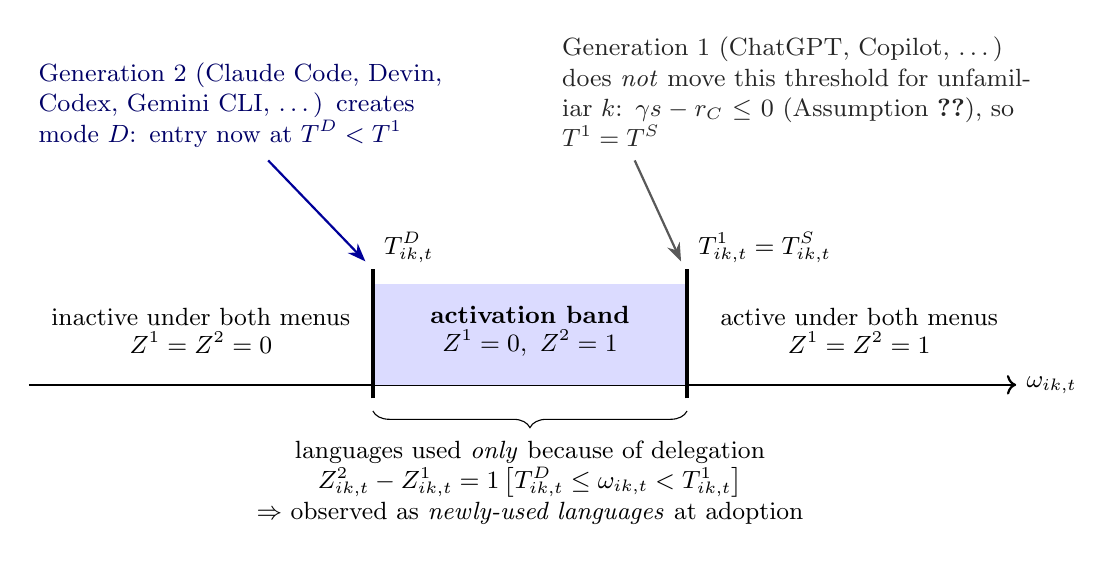
\begin{tikzpicture}[scale=0.95, every node/.style={font=\small}]
% ---- axis ----
\draw[->, thick] (0,0) -- (13.2,0)
  node[right, font=\small\itshape] {$\omega_{ik,t}$};
% ---- activation band shading ----
\fill[blue!14] (4.6,0) rectangle (8.8,1.35);
% ---- thresholds ----
\draw[very thick] (4.6,-0.18) -- (4.6,1.55);
\node[above right] at (4.62,1.5) {$T^D_{ik,t}$};
\draw[very thick] (8.8,-0.18) -- (8.8,1.55);
\node[above right] at (8.82,1.5) {$T^1_{ik,t}=T^S_{ik,t}$};
% ---- region labels ----
\node[align=center] at (2.3,0.72)
  {inactive under both menus\\[-1pt] $Z^1=Z^2=0$};
\node[align=center] at (6.7,0.72)
  {\textbf{activation band}\\[-1pt] $Z^1=0,\ Z^2=1$};
\node[align=center] at (11.1,0.72)
  {active under both menus\\[-1pt] $Z^1=Z^2=1$};
% ---- Gen-2 annotation (left threshold) ----
\node[align=left, anchor=south west, text width=5.5cm, blue!40!black]
  (gentwo) at (0.0,3.05)
  {Generation 2 (Claude Code, Devin, Codex, Gemini CLI, \ldots) creates
   mode $D$: entry now at $T^D < T^1$};
\draw[-{Stealth}, thick, blue!60!black] (3.2,3.0) -- (4.5,1.65);
% ---- Gen-1 annotation (right threshold) ----
\node[align=left, anchor=south west, text width=5.9cm, gray!30!black]
  (genone) at (7.0,3.05)
  {Generation 1 (ChatGPT, Copilot, \ldots) does \emph{not} move this
   threshold for unfamiliar $k$: $\gamma s - r_C \le 0$
   (Assumption \ref{ass:foothold}), so $T^1 = T^S$};
\draw[-{Stealth}, thick, gray!70!black] (8.1,3.0) -- (8.72,1.65);
% ---- brace under the band ----
\draw[decorate, decoration={brace, mirror, amplitude=6pt}]
  (4.6,-0.35) -- (8.8,-0.35);
\node[align=center, below] at (6.7,-0.62)
  {languages used \emph{only} because of delegation\\
   $Z^2_{ik,t}-Z^1_{ik,t} = \1{T^D_{ik,t}\le
   \omega_{ik,t} < T^1_{ik,t}}$\\
   $\Rightarrow$ observed as \emph{newly-used languages} at adoption};
\end{tikzpicture}
\end{singlespace}
\caption{The activation band for an unfamiliar language $k$, with the
tool generations of Section \ref{sec:background} placed on it.
Generation-1 tools leave the entry threshold at $T^1=T^S$ because their
value is proportional to skill the developer does not have in $k$;
Generation-2 tools add delegation, whose threshold $T^D$ does not
require language-specific skill. Opportunities falling in $[T^D, T^1)$
are produced only under menu $\mathcal{M}_2$ --- the model's prediction
for the spike in newly-used languages at first detectable Claude Code
use.}
\label{fig:band}
\end{figure}

\begin{remark}[What the model does and does not claim]
\label{rem:production-frontier}
The frontier in this model is a \emph{production} frontier, not a
\emph{skill} frontier. A language enters the active set when the
developer can profitably deliver work in it under \emph{some} mode in
her menu --- including delegation, in which the agent executes share
$\lambda$ while the developer specifies, decomposes, and verifies. The
model does not claim that adoption raises language-specific skill
$s_{ik,t}$: a developer who could only write Python solo may now ship a
Rust project, but by directing an agent, not by coding Rust unassisted.
Delegated output is nonetheless not autonomous machine output --- its
value $\lambda a_i z(A)$ is zero for a developer with no general
ability, and it carries the human verification cost $\kappa(a,s)$.
Skill acquisition enters only through the learning extension in
Appendix \ref{app:proofs}, which we treat as a secondary channel.
\end{remark}

\subsection{Flows versus stocks}

The band prediction concerns first uses, which are a \emph{flow}: a given
language can enter the portfolio only once. The corresponding \emph{stock}
is the cumulative count of languages ever used, and the two move
differently after adoption.

\begin{proposition}[Dynamic cumulative-language effect]
\label{prop:dynamic}
For an initially unfamiliar language, let $p^g_{ik}$ be the per-period
first-use hazard under generation $g$. If $p^2_{ik}\ge p^1_{ik}$, the
expected cumulative-language effect at event-time horizon $s$ is
\begin{equation}
\Delta C_i(s)
=
\sum_{k\in\mathcal{U}_i}
\left[
(1-p^1_{ik})^{s+1}-(1-p^2_{ik})^{s+1}
\right]\ge0,
\label{eq:cumulative-gap}
\end{equation}
which in the closed-frontier benchmark $p^1_{ik}=0<p^2_{ik}$ is strictly
increasing and concave over the observed horizon.
\end{proposition}

Newly-used languages may therefore spike at adoption and revert as the
at-risk set is depleted, while the cumulative stock keeps rising --- the
signature pattern the event studies test. Two extensions are developed in
Appendix \ref{app:proofs}: expected expansion is largest for high-ability
specialists, who combine many unfamiliar candidates with low verification
costs (Proposition \ref{prop:specialist}), and Bayesian learning from
agentic interaction can convert initially delegated languages into
persistent portfolio members by raising belief precision.

\subsection{Empirical mapping}

The model maps directly to the outcomes in Section \ref{sec:data}. The
monthly language count and language entropy capture the active-language
set of Equation \eqref{eq:expected-count}. Newly-used languages isolate
the activation band of Proposition \ref{prop:band}. Cumulative languages
correspond to the stock dynamics of Proposition \ref{prop:dynamic}.
Repository and commit counts are activity diagnostics rather than
frontier outcomes: they help establish that language expansion reflects
substantive new work, and they feed the volume-based robustness checks.
The specialist-heterogeneity prediction motivates a test by pre-adoption
portfolio breadth and ability proxies, carried out in Section
\ref{sec:mechanism}.
% === end archive member: sections/03_theory.tex ===
% === archive member: sections/10_appendix.tex ===
\section{Theory Appendix}
\label{app:proofs}

This appendix collects the derivations and proofs behind the propositions
in Section \ref{sec:theory}, states the specialist-heterogeneity and
learning extensions referenced there, and records the repository-expansion
result.

\subsection{CARA--Normal certainty equivalent}

Let a payoff $Y$ be conditionally Normal with mean $m$ and variance
$\sigma^2$, and let utility be $u(y)=-\exp(-\rho y)$ with $\rho>0$. The moment
generating function of the Normal distribution gives
\begin{equation}
\E[-\exp(-\rho Y)]
=-\exp\!\left(-\rho m+\frac{\rho^2\sigma^2}{2}\right).
\end{equation}
The certainty equivalent $\operatorname{CE}$ solves
$-\exp(-\rho\operatorname{CE})=\E[-\exp(-\rho Y)]$, hence
\begin{equation}
\operatorname{CE}
=m-\frac{\rho\sigma^2}{2}.
\label{eq:ce-formula-app}
\end{equation}
This is the mean-minus-risk-penalty expression used in the three production
modes.

\subsection{Threshold algebra}

Starting from the solo surplus
\[
V^S=\omega+s\mu-\frac{\rho s^2}{2\pi}-b,
\]
solo production is viable iff
\begin{equation}
\omega\ge T^S=b-s\mu+\frac{\rho s^2}{2\pi}.
\end{equation}
Generation-1 surplus is $V^C=V^S+\gamma s-r_C$, so its threshold is
\begin{equation}
T^C=b-s\mu-\gamma s+r_C+\frac{\rho s^2}{2\pi}
=T^S-(\gamma s-r_C).
\end{equation}
Because Generation 1 offers either solo or co-pilot production,
\begin{equation}
T^1=\min\{T^S,T^C\}=T^S-\max\{0,\gamma s-r_C\}.
\end{equation}
For an unfamiliar language, Assumption \ref{ass:foothold} implies
$\gamma s-r_C\le0$, so $T^1=T^S$.

Delegation is viable iff
\begin{align}
\omega\ge T^D
={}&
b-(1-\lambda)s\mu-\lambda a z(A)
+\kappa(a,s)+r_D
\nonumber\\
&\quad
+\frac{\rho}{2}
\left[
\frac{(1-\lambda)^2s^2}{\pi}
+\sigma_D^2(a,s,A)
\right].
\end{align}
For an unfamiliar language, the delegation advantage is $B=T^S-T^D$:
\begin{align}
B
={}&
\left(b-s\mu+\frac{\rho s^2}{2\pi}\right)
\nonumber\\
&-
\left\{
b-(1-\lambda)s\mu-\lambda a z(A)+\kappa(a,s)+r_D
+\frac{\rho}{2}
\left[
\frac{(1-\lambda)^2s^2}{\pi}
+\sigma_D^2(a,s,A)
\right]
\right\}
\nonumber\\
={}&
\lambda[a z(A)-s\mu]-\kappa(a,s)-r_D
+\frac{\rho}{2}
\left[
\frac{(2\lambda-\lambda^2)s^2}{\pi}
-\sigma_D^2(a,s,A)
\right],
\end{align}
which is Equation \eqref{eq:agentic-advantage} in the main text.

\subsection{Proof of Proposition \ref{prop:frontier}}

Because $\mathcal{M}_1=\{S,C\}\subset\{S,C,D\}=\mathcal{M}_2$,
\begin{equation}
V^2_{ik,t}
=\max\{V^S_{ik,t},V^C_{ik,t},V^D_{ik,t}\}
\ge
\max\{V^S_{ik,t},V^C_{ik,t}\}
=V^1_{ik,t}.
\end{equation}
If $V^1_{ik,t}\ge0$, then $V^2_{ik,t}\ge0$, so any language active under
Generation 1 remains active under Generation 2. If $V^1_{ik,t}<0$, then
$Z^1_{ik,t}=0$ and $Z^2_{ik,t}\in\{0,1\}$, so $Z^2_{ik,t}\ge Z^1_{ik,t}$.
Summing over languages gives $N^2_{it}\ge N^1_{it}$. Strict inequality holds
when at least one language is inactive under both old modes but active under
delegation. \hfill $\square$

\subsection{Proof of Proposition \ref{prop:band}}

For an unfamiliar language, Assumption \ref{ass:foothold} gives $T^1=T^S$.
If $B=T^S-T^D>0$, then $T^D<T^S$ and the Generation-2 threshold is $T^2=T^D$.
Thus
\[
Z^1=\1{\omega\ge T^S},
\qquad
Z^2=\1{\omega\ge T^D}.
\]
With $T^D<T^S$, these indicators differ exactly when
$T^D\le\omega<T^S$. Therefore
\[
Z^2-Z^1=\1{T^D\le\omega<T^S}.
\]
If $F$ is the conditional CDF of $\omega$, the probability of the band is
$F(T^S)-F(T^D)$. \hfill $\square$

\subsection{Specialist and ability heterogeneity}

The heterogeneity extension referenced in Section \ref{sec:theory} rests
on a symmetry assumption across unfamiliar-language candidates.

\begin{assumption}[Comparable unfamiliar-language candidates]
\label{ass:exchangeable}
Conditional on developer characteristics such as general ability, all
unfamiliar languages have the same per-language activation increment
$p_i(a_i,A)\ge0$, and $p_i$ is increasing in $a_i$ whenever Assumption
\ref{ass:verification} makes delegation thresholds fall with ability.
\end{assumption}

\begin{proposition}[Specialist and ability heterogeneity]
\label{prop:specialist}
Under Assumption \ref{ass:exchangeable}, expected expansion into initially
unfamiliar languages is
\begin{equation}
\E[E_i\mid a_i,U_i]=U_i p_i(a_i,A),
\qquad
E_i\equiv\sum_{k\in\mathcal{U}_i}(Z^2_{ik}-Z^1_{ik}).
\label{eq:specialist-expansion}
\end{equation}
It is increasing in the stock of unfamiliar-language candidates $U_i$ and
in general ability $a_i$. The largest extensive-margin gains accrue to
high-ability specialists.
\end{proposition}

\paragraph{Proof.}
Let $E_i=\sum_{k\in\mathcal{U}_i}(Z^2_{ik}-Z^1_{ik})$. Under Assumption
\ref{ass:exchangeable}, each unfamiliar language has the same activation
increment $p_i(a_i,A)$. Linearity of expectation gives
\begin{equation}
\E[E_i\mid a_i,U_i]
=
\sum_{k\in\mathcal{U}_i}\E[Z^2_{ik}-Z^1_{ik}\mid a_i]
=
U_i p_i(a_i,A).
\end{equation}
Because $U_i=K-|\mathcal{K}_i|$, a smaller familiar-language set mechanically
creates more unfamiliar-language candidates. Assumption \ref{ass:verification}
implies stronger general ability lowers verification costs and weakly lowers
residual error, so $p_i(a_i,A)$ is increasing in $a_i$ when the opportunity
density is positive at the relevant threshold. The product
$U_i p_i(a_i,A)$ is therefore largest for developers with many candidates and
high ability. \hfill $\square$

\subsection{Proof of Proposition \ref{prop:dynamic}}

For an initially unfamiliar language, under generation $g$ the probability of
no first use through horizons $0,\ldots,s$ is
\begin{equation}
\Pr(\mathcal{T}^g_{ik}>s)=(1-p^g_{ik})^{s+1}.
\end{equation}
Therefore the probability of at least one use by horizon $s$ is
\begin{equation}
\Pr(\mathcal{T}^g_{ik}\le s)=1-(1-p^g_{ik})^{s+1}.
\end{equation}
Summing over initially unfamiliar languages and subtracting generations gives
Equation \eqref{eq:cumulative-gap}. If $p^2_{ik}\ge p^1_{ik}$, then
$1-p^2_{ik}\le1-p^1_{ik}$, so each summand is nonnegative.

The first difference of the one-language cumulative gap is
\begin{align}
&\left[(1-p^1)^{s+2}-(1-p^2)^{s+2}\right]
-\left[(1-p^1)^{s+1}-(1-p^2)^{s+1}\right]
\nonumber\\
&\qquad
=
p^2(1-p^2)^{s+1}-p^1(1-p^1)^{s+1}.
\end{align}
Summing over languages, the effect grows between horizons $s$ and $s+1$
if and only if the no-catch-up condition
\begin{equation}
\sum_{k\in\mathcal{U}_i}
\left[
p^2_{ik}(1-p^2_{ik})^{s+1}
-p^1_{ik}(1-p^1_{ik})^{s+1}
\right]\ge0
\label{eq:no-catchup}
\end{equation}
holds. If $p^1=0<p^2$, the first difference is
$p^2(1-p^2)^{s+1}>0$ and the second difference is
$-(p^2)^2(1-p^2)^{s+1}<0$, giving strict increase and concavity.
\hfill $\square$

\subsection{Learning after agentic interaction}

The delegation channel explains why an unfamiliar language can be used
immediately; interaction with the agent and the language can also generate
learning that makes the language persist in the portfolio. Suppose the
developer observes signals
\begin{equation}
x_{\ell}=\theta_{ik}+\varepsilon_{\ell},
\qquad
\varepsilon_{\ell}\sim\N(0,\sigma_{\ell}^2),
\qquad
\ell=1,\ldots,L,
\label{eq:signals}
\end{equation}
conditionally independent given $\theta_{ik}$. Let
$q=\sum_{\ell=1}^L1/\sigma_{\ell}^2$ be the total signal precision and
$\bar{x}_q=(\sum_{\ell}x_\ell/\sigma_\ell^2)/q$ the precision-weighted
signal mean. The posterior kernel is proportional to
\[
\exp\left\{
-\frac{1}{2}\pi(\theta-\mu)^2
-\frac{1}{2}\sum_{\ell=1}^L\frac{(x_\ell-\theta)^2}{\sigma_\ell^2}
\right\},
\]
and collecting terms in $\theta$ gives the Bayesian update
\begin{equation}
\pi'_{ik}=\pi_{ik}+q,
\qquad
\mu'_{ik}=
\frac{\pi_{ik}\mu_{ik}+q\bar{x}_q}{\pi_{ik}+q}.
\label{eq:bayes-update}
\end{equation}
Learning raises precision and updates the productivity belief, so an
initially delegated language can remain active in later months. We use
this channel to interpret persistence and cumulative expansion, but not
as the primary proof of immediate diversification: information can
reveal bad matches as well as good ones.

\subsection{Repository expansion}

\begin{proposition}[Repository expansion]
\label{prop:repos}
Suppose each repository requires at least one programming language and carries
an entry cost that is weakly decreasing when the developer can activate that
language. If agentic delegation weakly expands the active-language set, then
the expected number of repositories the developer can contribute to weakly
increases. It increases strictly when some repositories require languages in
the delegation activation band.
\end{proposition}

\begin{proof}
Let repository $r$ require language $\ell(r)$ and deliver opportunity value
$\Omega_{ir,t}$. Write its entry condition as
$\Omega_{ir,t}\ge c_r(\ell(r),g)$ under generation $g$, where
$c_r(\ell,2)\le c_r(\ell,1)$ whenever delegation weakly lowers the activation
threshold for language $\ell$. The repository indicator under Generation 2
therefore weakly exceeds the Generation-1 indicator for every repository
opportunity. Summing over repositories and taking expectations gives weak
expansion; strict expansion follows if the opportunity distribution places
positive mass on repositories whose required language lies in the activation
band. \hfill $\square$
\end{proof}

\section{Classifying the Tools into the Model's Production Modes}
\label{app:tools}

Table \ref{tab:classification} assigns the AI coding tools of Section
\ref{sec:background} to the model's production modes. The
classification criterion is the \emph{locus of execution}, taken from
each tool's own primary-source capability description, not model
quality or release date: a tool is mode $C$ if the developer must read,
adapt, place, and run every piece of output; it is mode $D$ if the tool
itself edits files, runs commands, and iterates on errors. The 2023
proto-agents are listed separately: they had mode-$D$ mechanics but not
the reliability to constitute a real production mode.

\begin{table}[H]
\caption{Classification of AI coding assistance into the model's
production modes. Mode $C$ tools augment execution the developer still
performs herself ($V^C = V^S + \gamma s - r_C$: value proportional to
existing skill $s$). Mode $D$ tools execute on the developer's behalf
($V^D$: value scales with general ability $a$, not language-specific
skill), which is what moves the entry threshold from $T^1$ to $T^D$.}
\label{tab:classification}
\begin{small}
\begin{singlespace}
\begin{description}[leftmargin=0.45cm,labelsep=0.4em,style=nextline]
\item[\emph{Generation 1 --- autocomplete copilots.}]
Deep TabNine (Jul 2019), GitHub Copilot (Jun 2021), Codeium (2022),
Ghostwriter (Oct 2022), CodeWhisperer (Apr 2023), and Cody (2023)
suggest the next lines or a whole function inside the IDE; the developer
accepts, adapts, and runs the output. These are mode-$C$ tools: they
lower $T^C$ only where skill $s$ is high.

\item[\emph{Generation 1 --- conversational assistants.}]
ChatGPT (Nov 2022), Bing Chat (Feb 2023), Claude (Mar 2023), Bard
(Mar 2023), and Copilot Chat (2023) write snippets, explain errors, and
answer questions in a chat window; the developer transfers everything
into her own environment. These are also mode-$C$ tools, with the same
foothold logic as Assumption \ref{ass:foothold}:
$\gamma s-r_C\le0$ for unfamiliar $k$.

\item[\emph{2023 proto-agents.}]
AutoGPT (Mar 2023), BabyAGI (Apr 2023), smol-developer (May 2023),
GPT-Engineer (Jun 2023), and Aider (mid-2023) had mode-$D$ mechanics
(file writes and iteration) on models that could not sustain them; on
SWE-bench, the best model resolved 1.96\% of tasks. Here $D$ exists, but
$z(A)$ is too low: $T^D>T^1$ for almost all $k$.

\item[\emph{Generation 2 --- agentic assistants.}]
Devin (Mar 2024), SWE-agent (Apr 2024), OpenHands (2024), Copilot
Workspace (Apr 2024), Replit Agent (Sep 2024), Cursor agent (Nov 2024),
Windsurf/Cascade (Nov 2024), Cline (2024), Jules (Dec 2024), Copilot
agent mode (Feb 2025), \textbf{Claude Code (Feb 2025)}, Codex CLI/agent
(Apr--May 2025), Gemini CLI (Jun 2025), and Kiro (Jul 2025) inspect the
repository, edit files, run commands and tests, read errors, and iterate
from a natural-language specification. These are high-$z(A)$ mode-$D$
tools: they create $T^D<T^1$ for unfamiliar $k$, the activation band.

\item[\emph{Adjacent app-builder agents.}]
v0 (Oct 2023), Bolt.new (Oct 2024), and Lovable (Nov 2024) turn a
natural-language specification into a deployed web application. They
have mode-$D$ economics but target non-developers, outside the GitHub
developer population studied here.
\end{description}
\end{singlespace}
\end{small}
\end{table}

Two features of the table do analytical work. First, the mode-$C$ rows
were all available to \emph{every} developer well before the treatment
window, so the pre-period counterfactual is genuinely
$\mathcal{M}_1$-with-mature-tools, not ``no AI.'' Second, the mode-$D$
rows other than Claude Code are exactly the set the competing-agent
screen of Section \ref{sec:data} removes: a developer already using
Devin or Cursor's agent before her first Claude commit already had menu
$\mathcal{M}_2$, so her Claude date would mismeasure the menu
expansion.

\section{Event-Study Support and Extended Pre-Trends}
\label{app:support}

The panel covers 28 months, but the displayable event-study window is
asymmetric by design. On the post side, with not-yet-treated controls,
one-month anticipation, and the last cohort adopting in January 2026
(period 25), group-time effects are estimable only through period 23,
so the earliest cohort reaches at most event time $e=+7$; later horizons
have no remaining comparison units. On the pre side, the earliest cohort
adopts in period 16, so all ten cohorts support pre-period diagnostics
back to $e=-12$ and beyond. Table \ref{tab:risksets} reports the number
of cohorts and developers contributing at each event time; the thinning
support at $e\ge 5$ explains the widening confidence intervals at long
horizons in the main figures.

\begin{table}[H]
\caption{Event-time risk sets: cohorts and developers contributing.}
\label{tab:risksets}
\centering
\begin{threeparttable}
\input{tables/table_cl_risksets}
\begin{tablenotes}\footnotesize
\item \emph{Notes.} A cohort $g$ contributes to event time $e$ when
$2 \le g+e \le 23$: the lower bound reflects the varying base period,
the upper bound the last period with not-yet-treated comparison units
under one-month anticipation (last cohort adopts in period 25).
Developer counts are cohort sizes in the estimation sample summed over
contributing cohorts.
\end{tablenotes}
\end{threeparttable}
\end{table}

Figure \ref{fig:extended-pretrend} extends the pre-period window of the
event study to a full year for the two headline diversity outcomes. All
eleven pre-anticipation coefficients ($e \in \{-12,\ldots,-2\}$) are
tightly estimated zeros for both outcomes, with every cohort
contributing at every point; the only non-zero pre-adoption coefficient
remains the anticipation month $e=-1$ discussed in Section
\ref{sec:results-pretrends}.

\begin{figure}[H]
\caption{Extended pre-period window ($e \in [-12, 7]$): programming
languages and language entropy.}
\label{fig:extended-pretrend}
\centering
\includegraphics[width=0.85\textwidth]{es_extended_pretrend.pdf}
\end{figure}

\section{Additional Data Construction Details}
\label{app:data}

\subsection*{Bot-account filter}

We exclude developers whose login matches any of the following case-insensitive
substrings, applied after lower-casing the login string: \texttt{[bot]},
\texttt{-bot}, \texttt{\_bot}, \texttt{bot-}, \texttt{dependabot},
\texttt{renovate}, \texttt{github-actions}, \texttt{codecov},
\texttt{greenkeeper}, \texttt{snyk}. The pattern correctly identifies standard
CI/CD bots and dependency managers; we do not attempt to detect bespoke
organizational bots that do not follow these conventions.

\subsection*{Stratification scheme}

The treated sample of 5{,}000 developers is allocated proportionally across the
six adoption-month strata from April through September 2025. Within each month,
the allocation is divided equally across three intensity tiers: \emph{low}
(5--10 Claude commits), \emph{medium} (11--50), and \emph{high} ($\geq51$).
The control sample of 5{,}000 not-yet-treated developers follows the same
stratification scheme, proportional across two adoption-quarter strata
(2025\,Q4 and 2026\,Q1) and equal across the three intensity tiers within each
quarter.

\subsection*{Contribution-API fetch (repository discovery input)}

Each developer's monthly activity is retrieved by querying the GitHub GraphQL
API's \texttt{user.contributionsCollection} endpoint with \texttt{from} and
\texttt{to} parameters set to the first and last calendar dates of each month.
Within each window we retrieve up to 100 repositories
(\texttt{maxRepositories: 100}) and the top 15 languages per repository ordered
by byte size. This fetch serves as one of the three repository-discovery
sources for the commit-level construction below; its language fields are used
only as a cross-check.

\subsection*{Commit-level construction}

The outcome data are built in three stages. \emph{Repository discovery}
unions three sources per developer: the contribution-API repositories
above; the repositories appearing in the raw Claude-commit stream; and
the GH~Archive record of public \texttt{PushEvent}s keyed to the
developer's login, queried on BigQuery over January 2024--April 2026.
Because push events fire for any branch and any authoring email, the
archive source adds 45 percent more (developer, repository) pairs than
the first two sources combined, for a total of 133{,}096 pairs.
\emph{Commit enumeration} lists all commits authored by the developer in
each discovered repository within the window via the REST commits
endpoint, yielding 3{,}151{,}624 distinct commits after de-duplicating
identical commits appearing in both forks and upstream repositories
(each commit is fetched once, preferring the developer's own
repository). \emph{File extraction} obtains each commit's changed file
paths and full commit message from bare, blob-filtered clones of each
repository (\texttt{git clone --bare --filter=blob:none}), reading the
commit graph with \texttt{git log --name-status} across all branches; a
per-SHA REST fallback recovers commits no longer reachable from any
branch after force-pushes. The procedure recovers changed-file records
for 99.997 percent of enumerated commits --- 3{,}151{,}536 commits
touching 57.2 million files. Merge commits are identified by parent
count and excluded from language construction. Each changed file is
assigned a language by GitHub Linguist's filename and extension rules
(exact filenames first, then extensions, ambiguous extensions resolved
to Linguist's popular default), retaining files classified as
\emph{programming} languages and applying Linguist's path-based
vendored, generated, and documentation exclusions. Claude co-authorship
is detected from the \texttt{Co-Authored-By: Claude} trailer in the
commit message; the same message scan detects the competing-agent
signatures listed in Section \ref{sec:data}.
% === end archive member: sections/10_appendix.tex ===
